
% \begin{wrapfigure}{r}{0.18\textwidth}
%     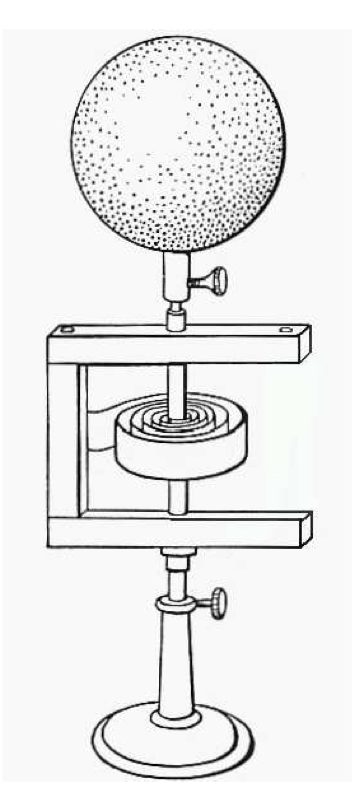
\includegraphics[width=0.14\textwidth]{Drillachse.jpeg}
%     %\caption{Drillachse (Q\cite{anleitungV101}).}
%     \label{fig:Drillachse}
% \end{wrapfigure}
% %\FloatBarrier
\section{Versuchsaufbau}
\label{sec:Versuchsaufbau}
Das Trägheitsmoment von verschiedenen Körpern wird mit Hilfe einer
Drillachse bestimmt. Dafür wird der Körper auf eine zweifach in einem Rahmen 
drehbare Achse besfestigt. Diese ist über eine Spiralfeder mit dem Rahmen 
verbunden. Nachdem die Winkelrichtgröße $D$ und das Eigenträgheitsmoment $I_{\text{Drill}}$
der Drillachse bekannt ist, lassen sich anhand der Schwingungsdauer $T$ der 
unterschiedlichen Körper die jeweiligen Trägbeitsmomente bestimmen.
%
\section{Durchführung}
\label{sec:Durchführung}
\subsection{Apparaturkonstanten der Drillachse}
\label{sec:Apparturkonstanten}
Die Winkelrichtgröße $D$ der Drillachse wird bestimmt, indem an dem Auslenkstab
ein Newtonmeter im einem Abstand von ca. $20\,\,\unit{\centi\meter}$ von der Mitte 
befestigt wird. Der Auslenkstab wird nun um den Winkel $\varphi$ ausgelenkt, wobei zu beachten ist,
dass das Newtonmeter senkrecht zum Stab ausgerichtet ist. Die aufzuwendene Kraft der Feder wird nun
für zehn verschiedene Winkel notiert. Für die Berechnung der Drillachse $I_{\text{Drill}}$ werden an beiden Seiten des 
Auslenkstabs Zylinder befestigt, welche den selben Abstand zur Mitte sowie ungefährt die selbe Masse und Größe
haben. Diese werden um $90°$ ausgelenkt und die fünffache Schwingungsdauer $5T$ wird gemessen. Diese Messung
wird jeweils für zehn verschiedene Abstände durchgeführt.
%
\subsection{Trägheitsmoment zwei verschiedener Körper}
\label{sec:TragheitZweiKörper}
Für die Bestimmung der Trägheitsmomente von zwei verschiedenen Körpern, werden die Körper an der Drillachse
befestigt und umd $90°$ ausgelenkt. Dabei wird zehnmal die fünfache Schwingungsdauer $5T$ gemessen. Anschließend
lassen sich die Trägheitsmomente der Körper mit der Winkelrichtgröße $D$ und der Eigenträgheitsmoment $I_{\text{Drill}}$ berechnen.
\subsection{Trägheitsmoment der Puppe}
\label{sec:TragheitPuppe}
%
Zunächst wird der Körper der Puppe gemessen. Hierzu werden die Beine, die Arme, der Körper und der Kopf in Zylinder
aufgeteilt. Daher werden die Höhe und der Durchmesser der einzelnen Körperteile gemeessen. Das Trägheitsmoment der Puppe wird 
für zwei verschiedene Körperstellungen bestimmt. Diese sind in der Abbildung (\ref{fig:BilderPuppe}) zu erkennen. Für die erste Position sind die Arme der Puppe horizontal ausgestreckt. 
Für die zweite Position sind zusätzlich die Beine in einem Winkel von $90°$ ausgestreckt. Für beide Körperhaltungen wird 
die Puppe um $90°$ ausgelenkt und jeweils fünfmal die fünffache Schwingungsdauer $5T$ gemessen. Zusätzlich wird die Puppe 
in beiden Positionen um $120°$ ausgelenkt und dabei wird erneut jeweils fünfmal die fünffache Schwingungsdauer $5T$ gemessen. 
%
% \begin{figure}
%     \centering
%     \begin{minipage}{.5\textwidth}
%       \centering
%       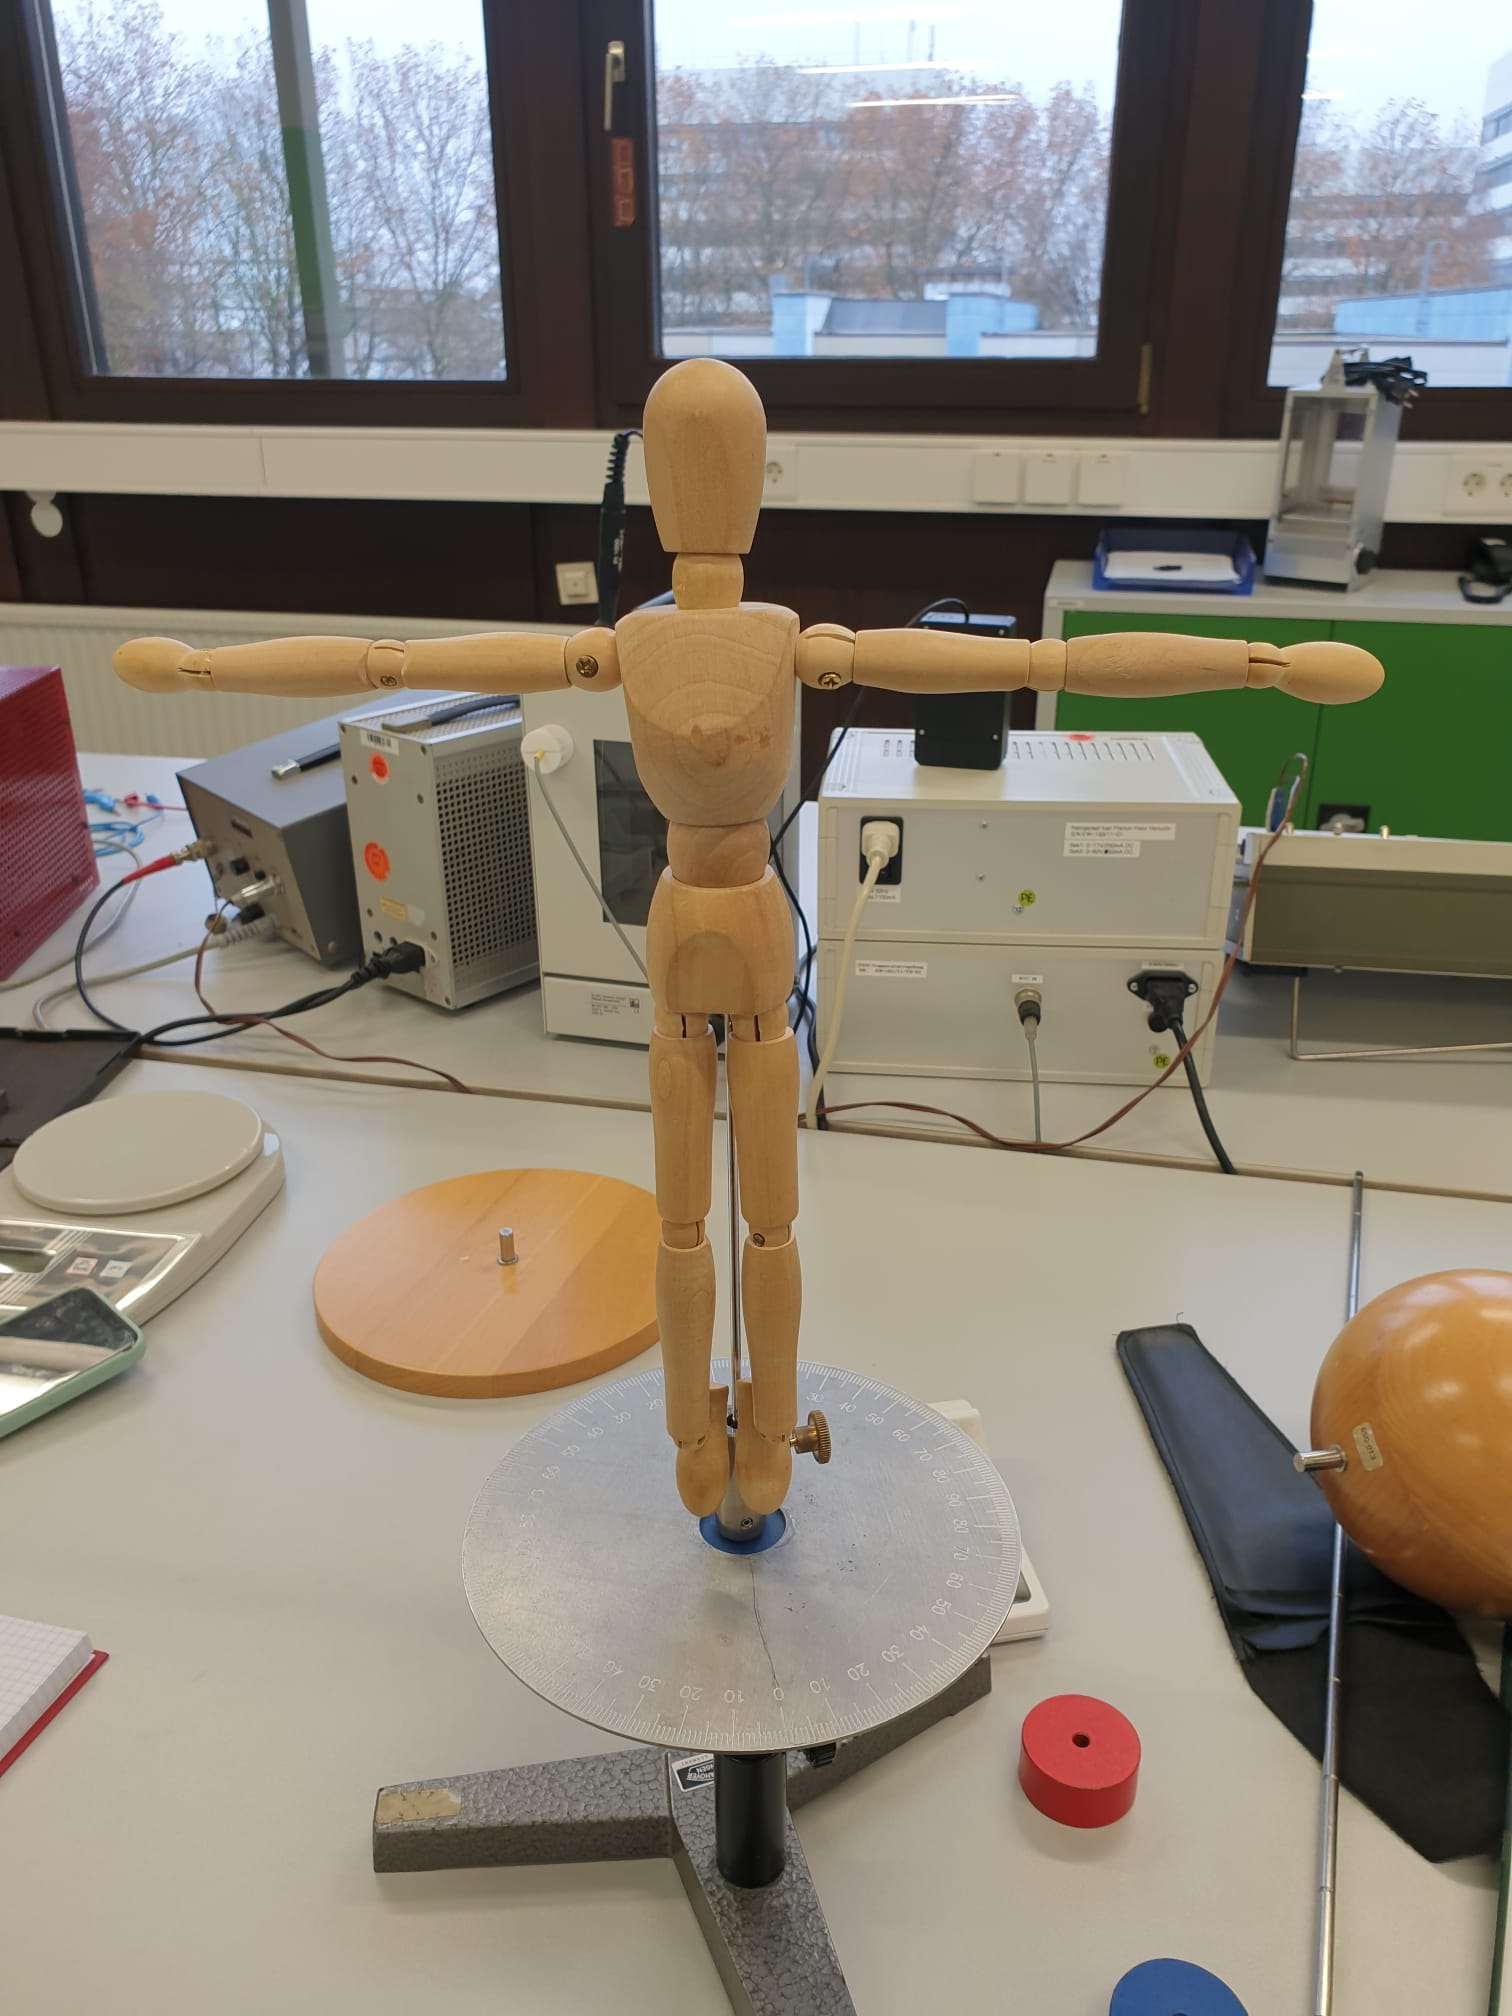
\includegraphics[width=.6\textwidth]{Position_1.jpeg}
%       \captionof{figure}{1. Position der Puppe}
%       \label{fig:ErstePosition}
%     \end{minipage}%
%     \begin{minipage}{.5\textwidth}
%       \centering
%       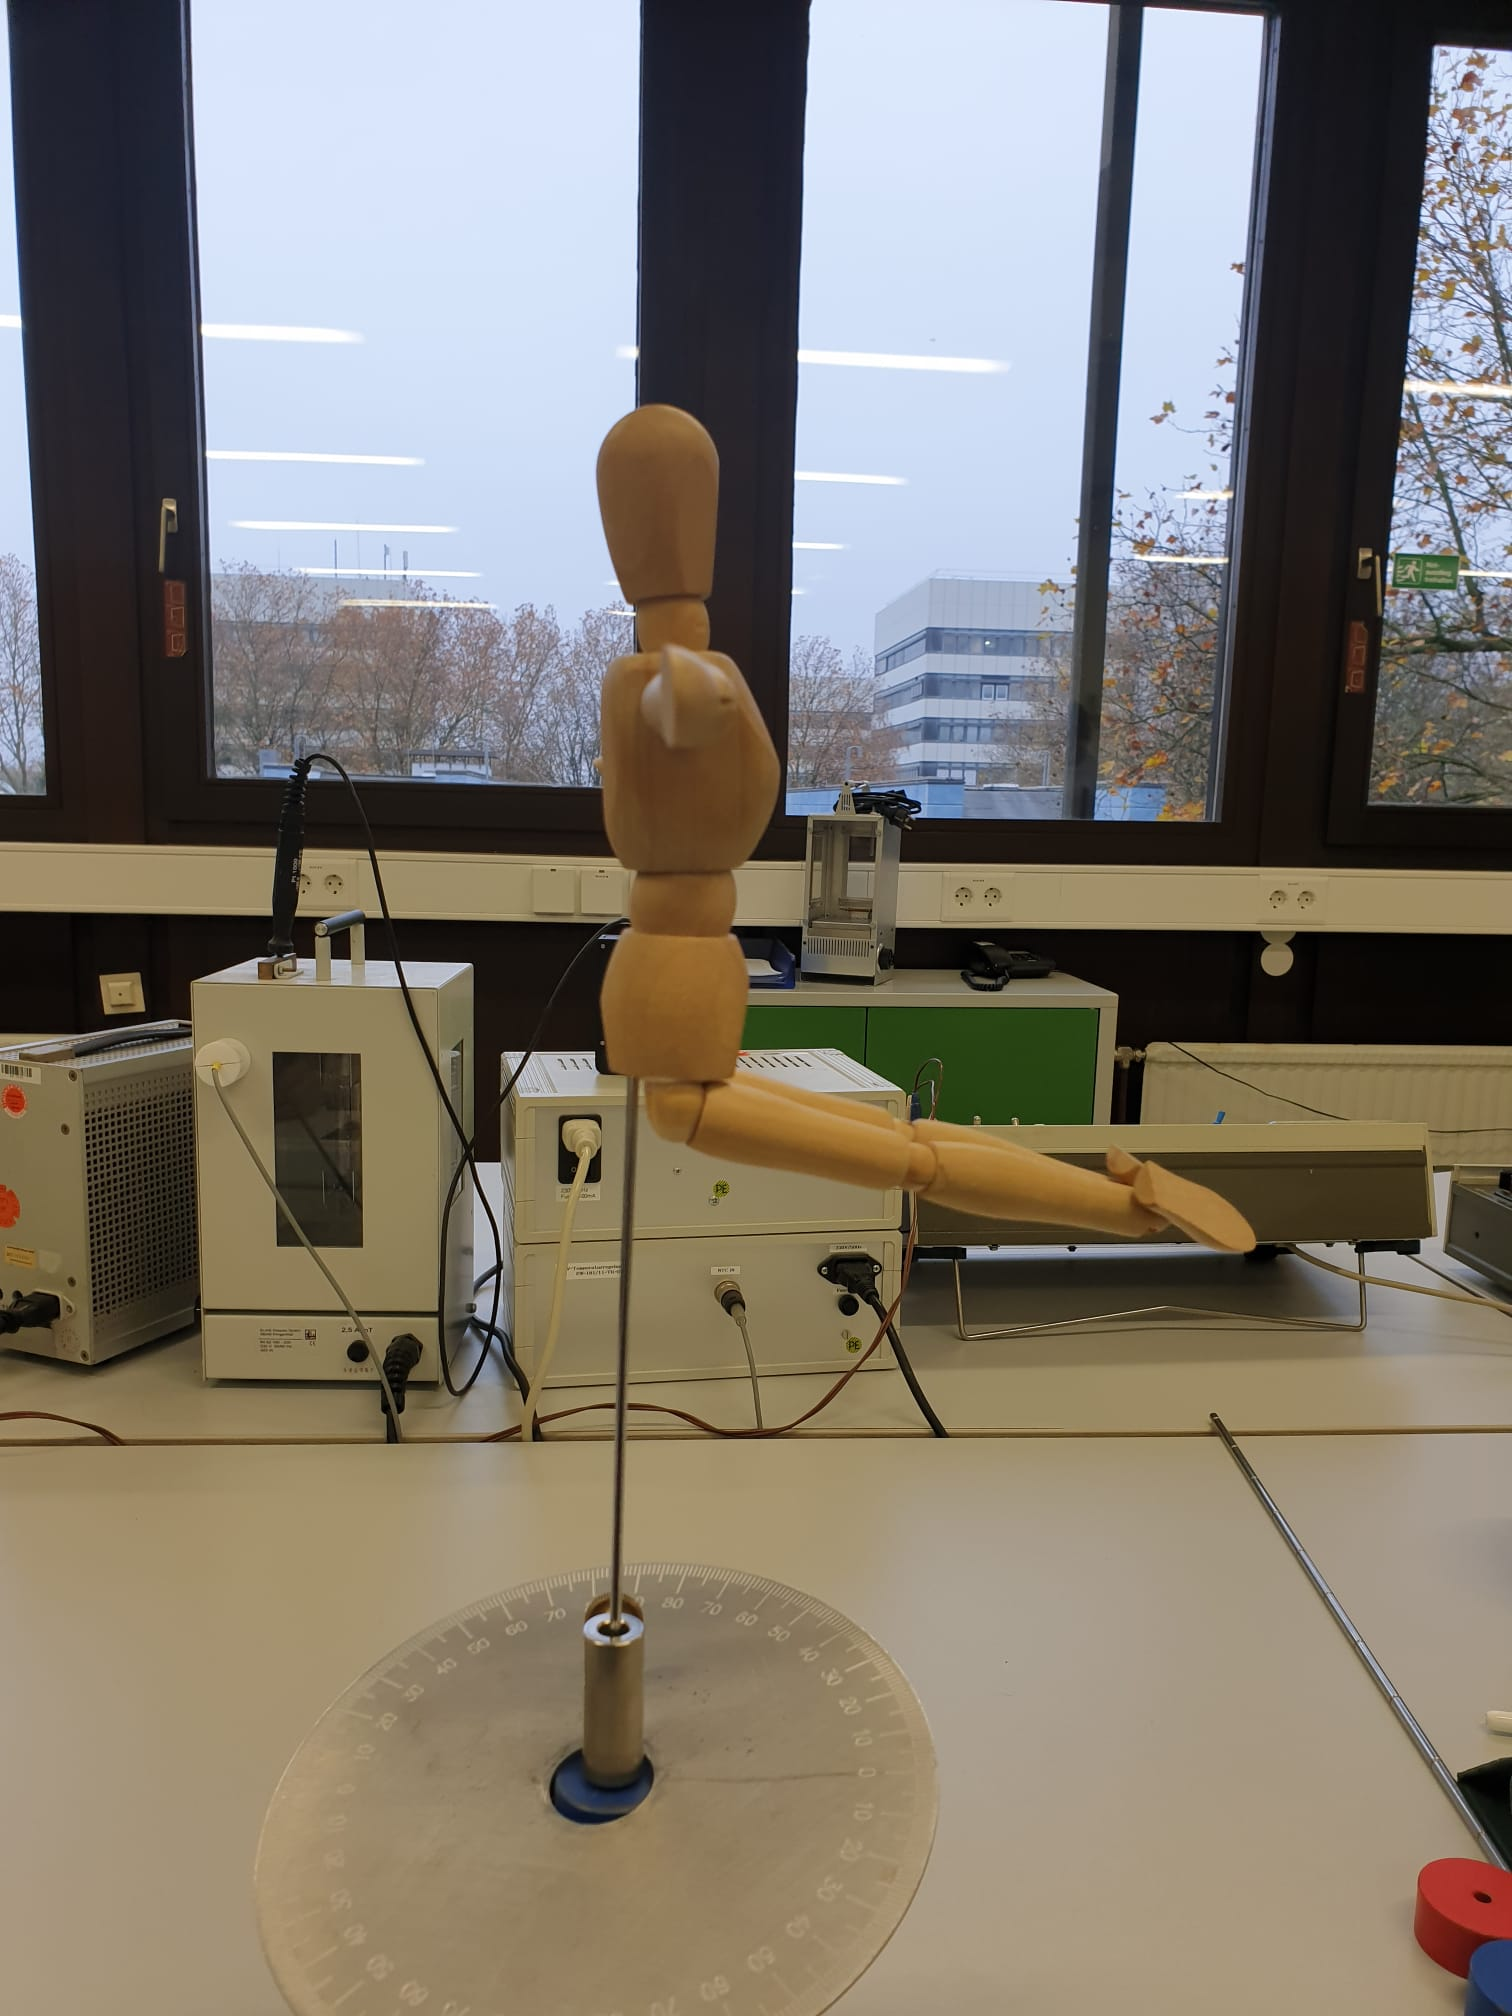
\includegraphics[width=.6\textwidth]{Position_2.jpg}
%       \captionof{figure}{2. Position der Puppe}
%       \label{fig:ZweitePosition}
%     \end{minipage}
% \end{figure}
\begin{figure}
    \centering
    \begin{subfigure}{0.5\textwidth}
      \begin{center}
      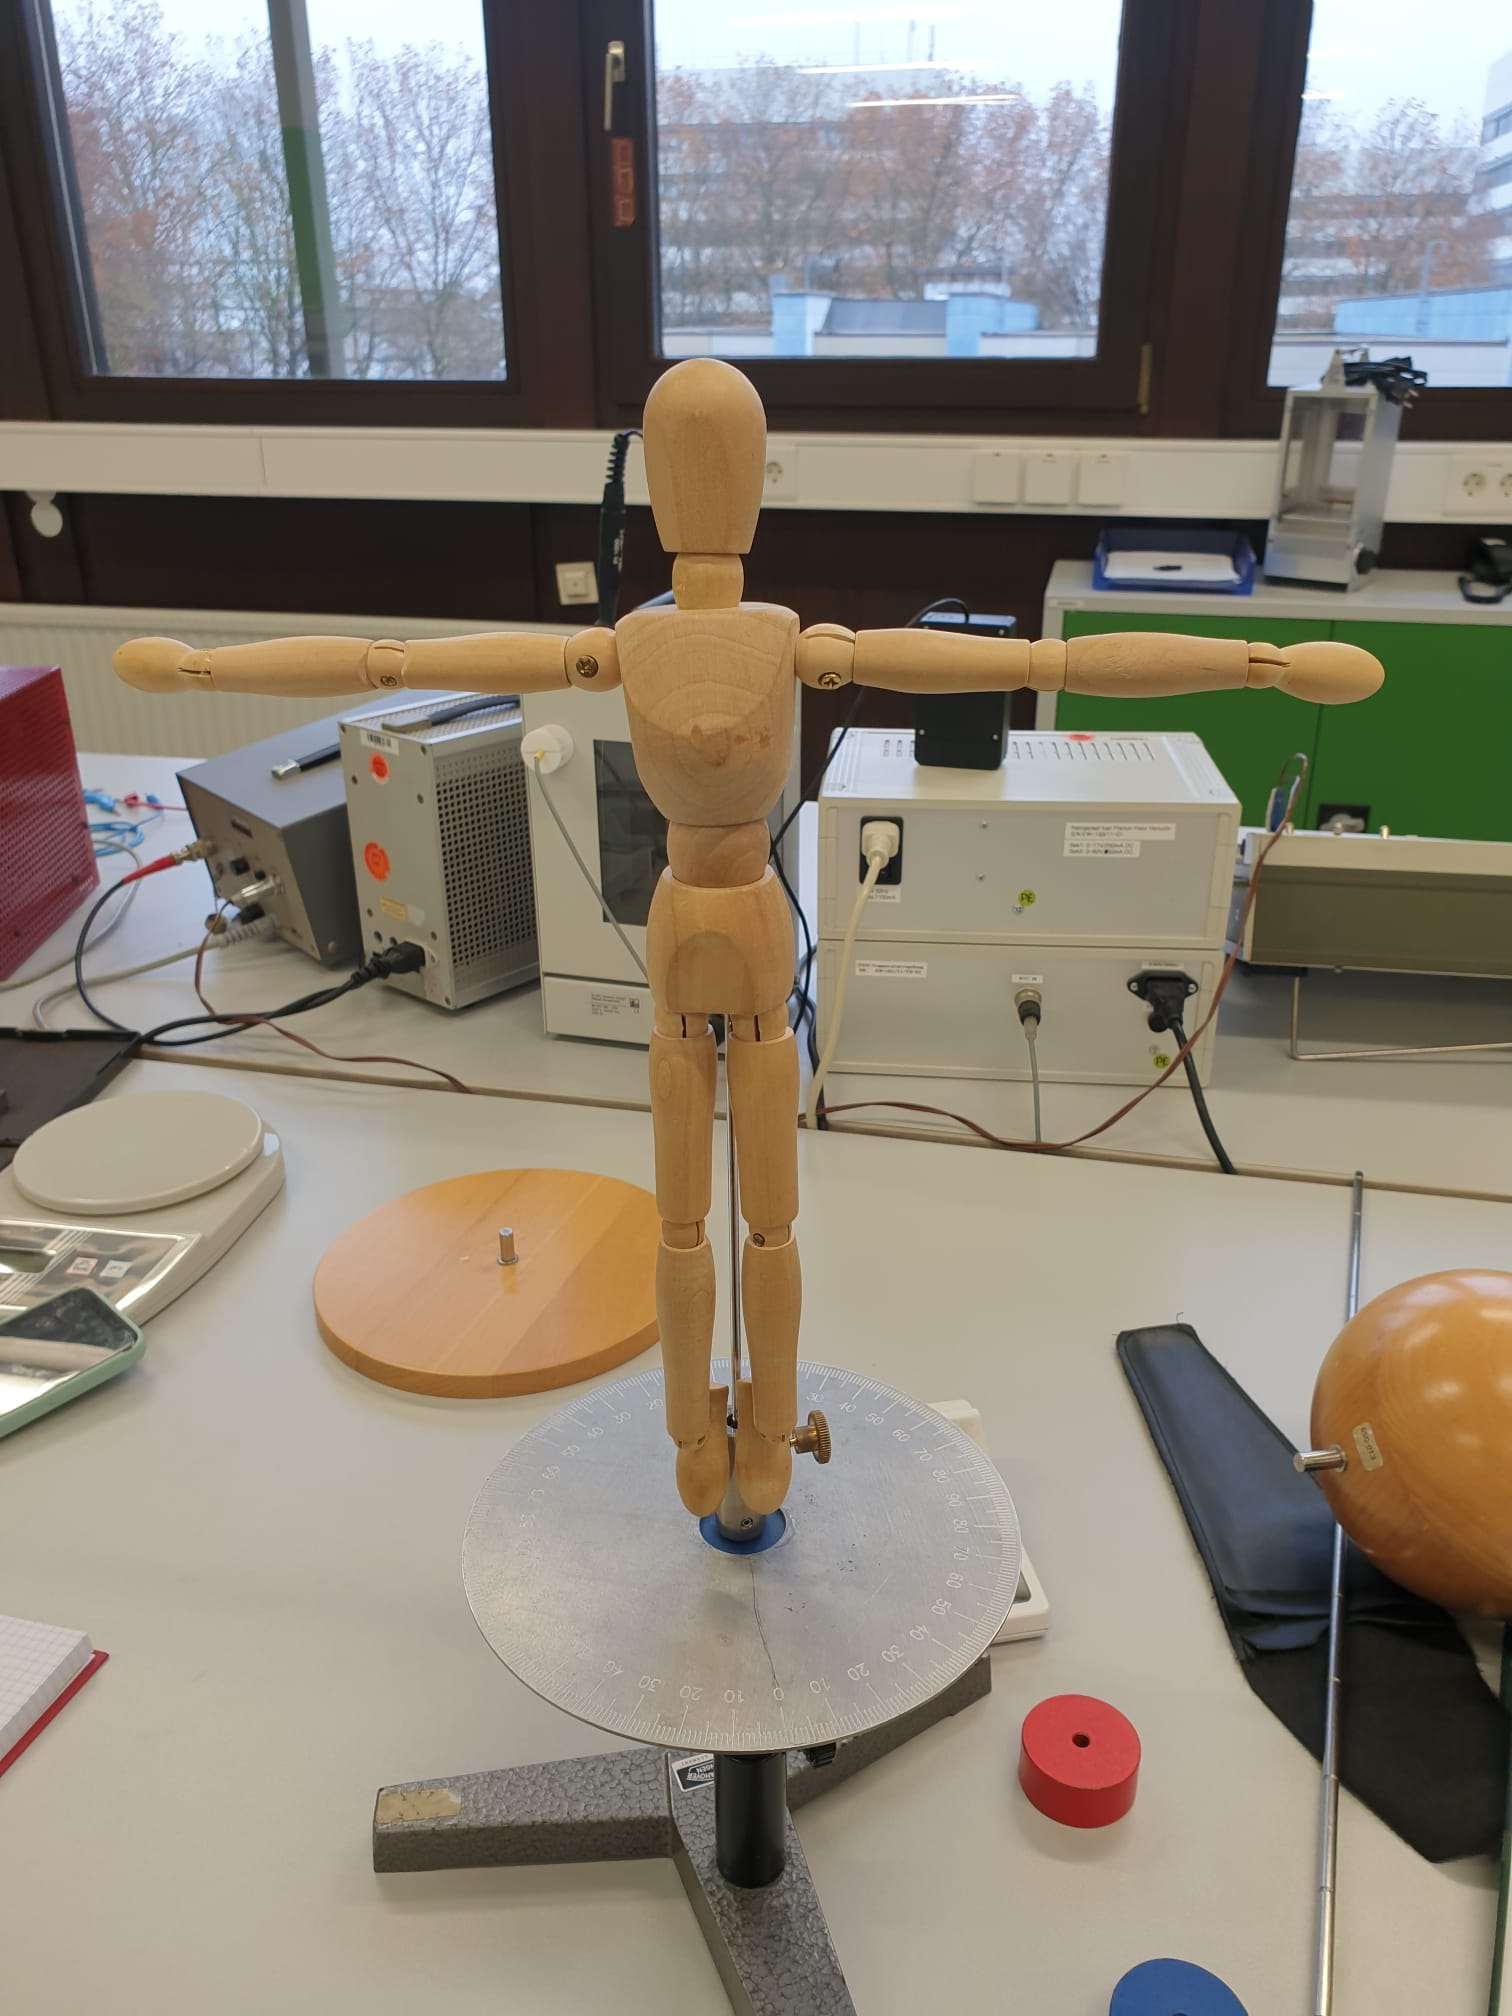
\includegraphics[width=0.7\textwidth]{Position_1.jpeg}
      \caption{Position 1 der Puppe.}
      \label{fig:sub1}
      \end{center}
    \end{subfigure}%
    \begin{subfigure}{0.5\textwidth}
      \begin{center}
      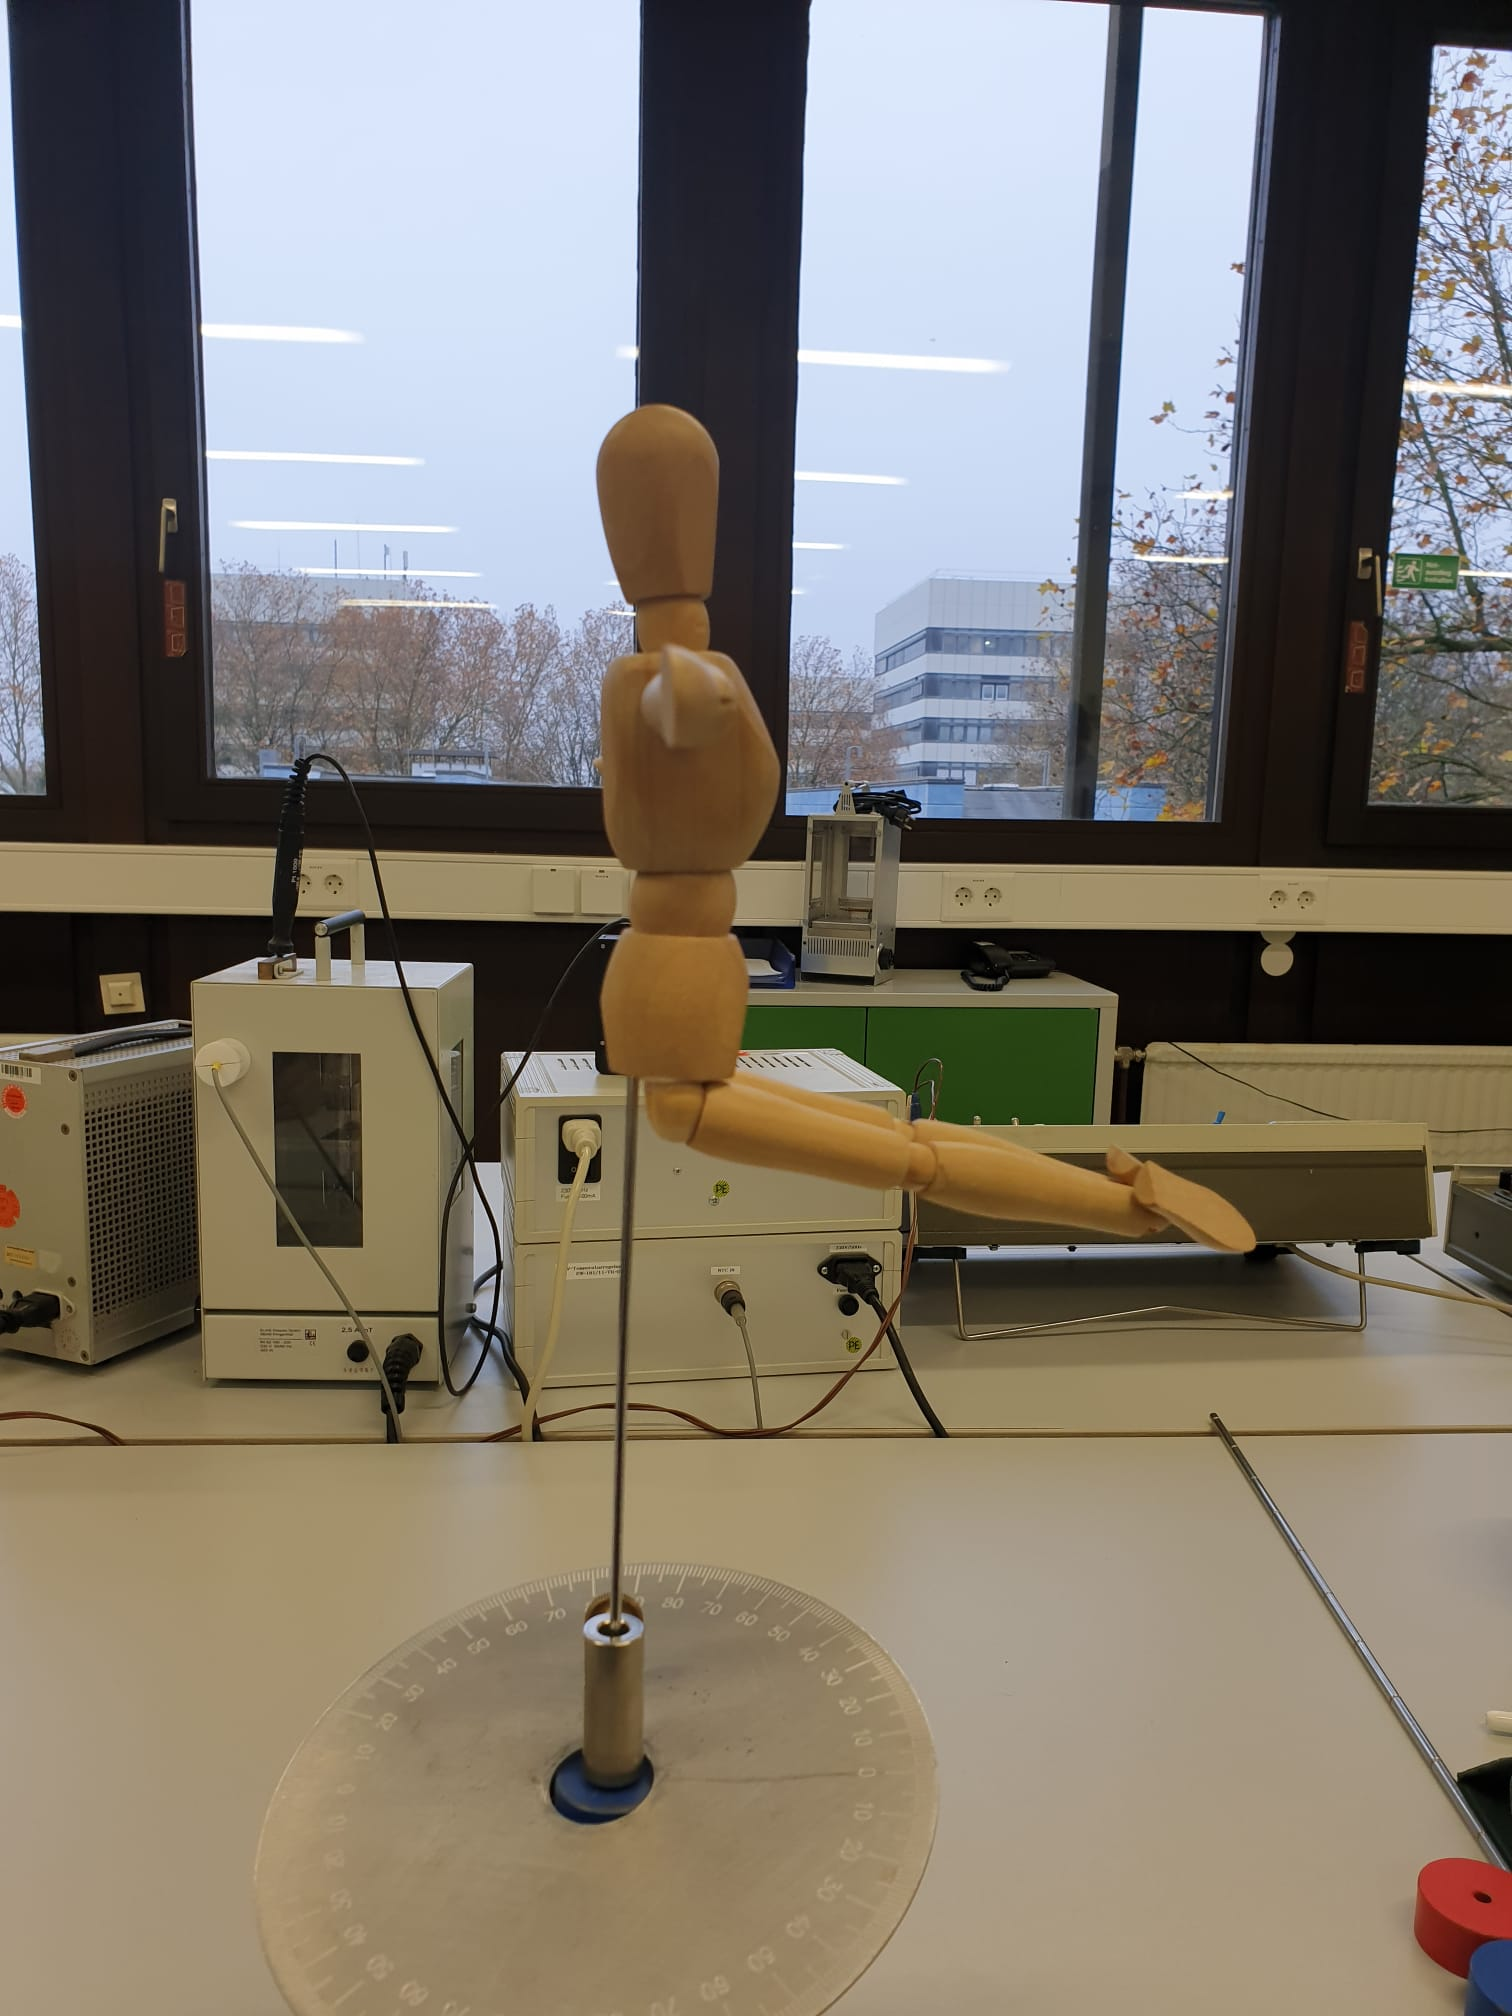
\includegraphics[width=0.7\textwidth]{Position_2.jpg}
      \caption{Position 2 der Puppe.}
      \label{fig:sub2}
      \end{center}
    \end{subfigure}
    \caption{Bildliche Darstellung der beiden Körperhaltungen der Puppe.}
    \label{fig:BilderPuppe}
\end{figure}